\section{Introduction}
As services are often developped around virtualization, vulnerabilities in hypervisors can now
have critical impact on businesses.

\subsection{Virtualization Evolution}
Virtualization has become a big part of the business in IT environment because 
of it's flexibility and optimization of performance, example instead of using one physical
machine of each employee, the  company can have a centralized data center and the
employee could open his session in every terminal available in the company.

 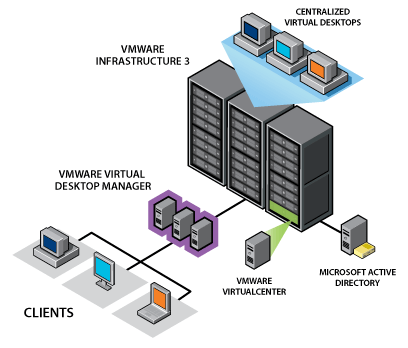
\includegraphics {vdivdm_diagram.png}

This kind of approach will improve flexibility, reliability, and security,
 but this kind of environment come with some security questions we'll discuss in this paper.

The companies take for granted that this new approach is better and more secure,
so the use of this technologies rises twice every year as a marketing study made by
Gartner IT infrastructure Operations and Management Summit in 2010, and in the top
of this market is Vmware products and for the open source solution we have Qemu/KVM.
I the other hand one study made by IBM in 2010 prove that this technologies are not unbreakable
and the study show many types of vulnerabilities, but we concentrate in the hypervisors and
try to answer two questions:
\begin{description}
\item[Escape to host] This vulnerability allow an attacker to have access to some resources
in the host where the virtual machine is, like cpu time, hard drive and memory.
\item[Escape to hypervisor] This vulnerability allow the attacker not to have direct access
to the host resources as the last one but, the attacker can still having access to the resources
of other virtual machines in the same host, compromising privacy and confidential data of other users.
\end{description}

\subsection{Impact of hypervisor vulnerabilites}
There are many ways to acces a virtual machine, through other vulnerabilities of
the softwares which are running inside of the virtual machine or through
usage of a public service (e.g. VPS provided by \emph{Rackspace} or instances
provided by \emph{Amazon EC2}).
In our study, we assume that the attacker has access to a virtual machine
running on top of a shared host.

If an attacker is able to find a vulnerabilitie in the hypervisor, it may have
terrible consequence on the other virtual machines :
\begin{description}
\item[Denial of Service] If the attacker is able to crash the hypervisor or part
of it, he could impact all the virtual machine running on top of it.
\item[Data leak] If an attacker is able to read arbitrary location in the memory
or hard drive of the hypervisor, he could steal business critical information.
Even through an attacker can't find a way to execute code he can still have
access of some resources like the hard drive and the attacker can steal
other users information or sensitive data.
\item[Control flow hijacking] This case would be the worst one. If the attacker
is able to execute arbitrary code in the host, he would have access of all
resources in the host, including the ressources of the other virtual machines.
This would allow him to access data, crash the other virtual machines but also
execute more subtle attacks.
\end{description}

These type of attacks are widely documented in the litterature, the main point is
that vulnerabilities at the hypervisor level may impact the host but also the other
virtual machines running on the hypervisor.

\subsection{Aim}
We think that we may answer the following questions :
\begin{itemize}
\item Are there similarities in the vulnerabilites which were already disclosed ?
\item Are the recent discolsed vulnerabilities exploitable to gain access to host
ressources from the guest ?
\item Can we easily find new vulnerabilities ?
\item How can we detect or prevent them ?
\end{itemize}

\section{Study case}

For our study we use the KVM public bug trackers and for Vmware we didn't be able
to use the bug tracker, because its private, but we can still have access to the CVEs
and some others less trusted sources, like forums and unofficial bug trackers,
we concentrate our research in two specific cases can we have access to the host
resource, or even control the host, or at least being able to have access to the resources
or even take control of other virtual machines in the same host.
Also for this research we use two types of virtualiazation:
\begin{description}
\item[Workstation] The workstation approach like vmware workstation, is meant 
to development of virtual infrastructure or personal and small business use. The advantage 
is easy and more flexible to use, but in the other hand scalability is totally lost.
\item[Server] The server approach is meant to big data center, for medium and big companies,
in this approach the scalability is easy, the migration, backup, and load balancing are very important
in difference to the workstation approach. In the other hand is not that easy to use, and deployment
of the physical infrastructure is not easy at first.
\end{description}

\section{Awaited result}

Our research show that products like vmware still having some vulnerabilities but 
more the software become old less critical vulnerabilities like control hijacking are found,
the same case is for Qemu/KVM, in the other hand we have also the hardware effort to
improve the trusted computing base, so it's more difficult to control the hypervisor or even
the host, but resent vulnerabilities in Vmware work station for example sharing folders
between the host and the virtual machines showed that an attacker could exploit a vulnerability
in this protocol and had access to all the folders in the host machine and not only the one was
specified by the administrator.
In a similar case we have KVM and sharing the network card could lead an attacker to create
a denial of access in the ethernet device and make unreachable by ethernet other virtual machines
sharing the same ethernet devices. 
